\section{Обзор существующих работ и решений}
\label{section.theory}
% \subsection{Маркетплейсы}
На данный момент существует большое количество NFT маркетплейсов: opensea \cite{opensea}, rarible \cite{rarible}, solanart \cite{solanart}. Если брать маркетплейсы только на базе NEAR Protocol, тогда существуют такие примеры как: paras \cite{paras}, mintbase \cite{mintbase}. Остановимся на них поподробнее.

\subsection{Paras}
\label{section.theory.paras}

Paras является наиболее популярным, интерфейс взаимодействия представлен пользователю в веб-браузере по адресу paras.id. Для того, чтобы авторизоваться нужно использовать
предоставить свой NEAR кошелек. Paras предоставляет огромное количество функций:
\begin{enumerate}
    \item Создать NFT токен.
    \item Выставить на продажу NFT токен.
    \item Обновить цену выставленному на продажу NFT токену.
    \item Убрать с продажи выставленной NFT токен.
    \item Уничтожить свой NFT токен.
    \item Получить продаваемые NFT токены со следующей фильтрацией:
        \begin{enumerate}
            \item Фильтрация по содержимому токена (картинки) - пиксель арт, фотографии, иллюстрации и так далее.
            \item Фильтрация по времени создания.
            \item Фильтрация по максимальной цене.
            \item Фильтрация по минимальной цене.
        \end{enumerate}
    \item Выставить оффер на непродаваемый токен.
\end{enumerate}

Smart-контракты Paras лежат в открытом доступе \cite{parasnftcontract, parasmarketplacecontract}.

\begin{remark}
    Обычно smart-контракты DApps принято выкладывать в открытый доступ, чтобы любой пользователь мог их посмотреть и полностью доверять сервису.
\end{remark}

С точки зрения написания smart-контрактов Paras имеет абсолютно такую же структуру NFT smart-контракта, потому что они придерживаются стандарта \cite{nftstandart} (см. {\color{blue} \ref{section.main.smart.struct}}).
Дополнительно они привязывают каждый токен к какой-то конкретной коллекции и не позволяют создавать токен без привязки к коллекции (Рисунок {\color{blue} \ref{fig.parascollections}}).

\begin{figure}
	\centering
	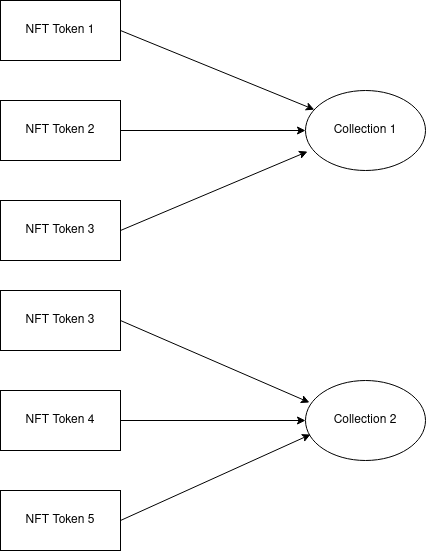
\includegraphics[height=60mm]{fig/parascollections.png}
	\caption{NFT токены и колекции в paras}
    \label{fig.parascollections}
\end{figure}

Smart-контракт маркетплейса paras предоставляет дополнительную функцию, как выставление оффера (предложения о покупке) на любой NFT токен. Эту функцию мы планируем позаимствовать в ближайшем будущем.

% \begin{listing}
% \begin{minted}[breaklines,fontsize=\scriptsize]{js}
% {
%     token_id: "304990:24",TokenSeriesJson
%     owner_id: "maxzeinly.near",
%     metadata: {
%         title: "Proof of Attendance No.1 #24",
%         description: null,
%         media: "bafybeib3c3r7vjbmyetawahj4kprei6satcrq23k2qjlx2gnmxmv5c6lza",
%         media_hash: null,
%         copies: 1111,
%         issued_at: "1652813800358071368",
%         expires_at: null,
%         starts_at: null,
%         updated_at: null,
%         extra: null,
%         reference: "bafkreiai54itp2hf267leg6754xmlst6j5m3yp3sin6n5bgva2q44wwtem",
%         reference_hash: null
%     },
%     approved_account_ids: {}
% }
% \end{minted}
% \caption{Структура NFT}
% \end{listing}

Paras, как и большинство маркетплейсов хранит медиа-файл и метаданные NFT на IPFS \cite{ipfs} (см. {\color{blue} \ref{section.main.bot.storage}}). IPFS предоставляется сервисом fleek \cite{fleek}. В качестве ссылки на медиа-файл и метаданные они хранят CID, а не полный URL, это связанно с тем, что минт NFT таким образом будет гораздо дешевле, ведь хранение в NEAR, довольно дорогое (см. {\color{blue} \ref{section.main.bot.struct}}). URL восстанавливается с помощью вызова метода <<nft\_metadata>> у NFT контракта для получения нужного шлюза (Листинг {\color{blue}\ref{lst.parasnftmetadatastruct}}), а после CID подставляется в URL этого шлюза (Листинг {\color{blue}\ref{lst.pastecidnearwallet}}), где при неуказании берется шлюз от cloudflare, который по опыту слабодоступен.

\begin{listing}
\begin{minted}[breaklines,fontsize=\scriptsize]{js}
function buildMediaUrl(media, base_uri) {
    if (!media || media.includes('://') || media.startsWith('data:image')) {
        return media;
    }
    if (base_uri) {
        return `${base_uri}/${media}`;
    }
    return `https://cloudflare-ipfs.com/ipfs/${media}`;
}
\end{minted}
\caption{Подстановка CID в URL у NEAR Wallet \cite{pastecidnearwallet}}
\label{lst.pastecidnearwallet}
\end{listing}

\begin{listing}
\begin{minted}[breaklines,fontsize=\scriptsize]{js}
{
    spec: 'nft-1.0.0',
    name: 'Paras Collectibles',
    symbol: 'PARAS',
    icon: "data:image/svg+xml,%3Csvg width='1080' height='1080' viewBox='0 0 1080 1080' fill='none' xmlns='http://www.w3.org/2000/svg'%3E%3Crect width='1080' height='1080' rx='10' fill='%230000BA'/%3E%3Cpath fill-rule='evenodd' clip-rule='evenodd' d='M335.238 896.881L240 184L642.381 255.288C659.486 259.781 675.323 263.392 689.906 266.718C744.744 279.224 781.843 287.684 801.905 323.725C827.302 369.032 840 424.795 840 491.014C840 557.55 827.302 613.471 801.905 658.779C776.508 704.087 723.333 726.74 642.381 726.74H468.095L501.429 896.881H335.238ZM387.619 331.329L604.777 369.407C614.008 371.807 622.555 373.736 630.426 375.513C660.02 382.193 680.042 386.712 690.869 405.963C704.575 430.164 711.428 459.95 711.428 495.321C711.428 530.861 704.575 560.731 690.869 584.932C677.163 609.133 648.466 621.234 604.777 621.234H505.578L445.798 616.481L387.619 331.329Z' fill='white'/%3E%3C/svg%3E",
    base_uri: 'https://ipfs.fleek.co/ipfs',
    reference: null,
    reference_hash: null
}
\end{minted}
\caption{Структура при вызове <<nft\_metadata>> у NFT контракта}
\label{lst.parasfunctioncallnftmetadata}
\end{listing}

Давайте рассмотрим структуру метаданных NFT (Листинг {\color{blue}\ref{lst.parasnftmetadatastruct}}). Paras, хоть и поддерживает по стандарту NEP-171 поле <<description>>, но хранит описание в метаданных NFT токена. Это аналогично тем же причинам, что и при хранении CID, а не полного URL в полях на медиа-файл и метаданные. Также они хранят название и идентификатор коллекции, создателя NFT, атрибуты и тип файла. Во многом наши метаданные будут подражать этой структуре.

\begin{listing}
\begin{minted}[breaklines,fontsize=\scriptsize]{json}
{
    "description":"Proof of Attendance to events hosted by NEAR Gang Couture.",
    "collection":"Haute Gang - Collaborations",
    "collection_id":"haute-gang-collaborations-by-neargangcouturenear",
    "creator_id":"neargangcouture.near",
    "attributes":[
        {"trait_type":"Rarity","value":"No Star"},
        {"trait_type":"Type","value":"Mask"}
    ],
    "blurhash":"UqFtJxPWpdyDGJ${t2V[?[ICMyenPCxVobae",
    "mime_type":"image/jpeg"
}
\end{minted}
\caption{Структура метаданных NFT в Paras}
\label{lst.parasnftmetadatastruct}
\end{listing}


\subsection{Mintbase}

Mintbase является менее популярным маркетплейсом, однако он предоставляем гораздо больше категорий NFT, но все ключевые функции такие же. В качестве новых категорий выступают: 3D изображение, gif, профессиональные фотографии, аудиодорожки, произведения художников.

Smart-контракты Mintbase на половину открыты (некоторые в открытом доступе, некоторые нет) \cite{mintbasecontracts}. С высокоуровневой точки зрения контракты Mintbase обладают совершенно другой архитектурой в отличие от Paras, так как в них вводится новый уровень абстракции.
Mintbase поддерживает структуру состающую из следующих взаимосвязанных сущностей: Store, Thing, Token.
\begin{enumerate}
    \item Store - NFT smart-контракт (децентрализованное API).
    \item Thing - тип NFT (коллекция токенов).
    \item Token - определенная NFT с уникальным владельцем.
\end{enumerate}
Касательно Thing, Token - все понятно, это просто коллекция и токен из конкретной колекции, а вот Store - обозначает магазин, который может выпускать колекции с токенами.
Чтобы пользователю начать создавать/продавать NFT ему нужно сначала создать свой Store smart-контракт. Для этого mintbase написала Factory библиотеку для создания своих Store.
После этого владелец от лица своего Store сможет создавать новые NFT токены и коллекции токенов.

Резюмируя, получается что пользователь создает свой маркетплейс контракт и использует его для покупки/продажи/создания с другими маркетплейс контрактами пользователей. Paras в свою очередь дает один уникальный маркетплейс контракт с которым взаимодействуют пользователи.

Mintbase хранит метаданные NFT в Arweave. Как уже говорилось, Mintbase очень сильно отошел от стандарта, что проявляется и выдаваемой структуре. Разницу можно заметить в полях <<metadata>>, <<royalty>> (см. {\color{blue} \ref{section.main.smart.struct.royalties}}) и <<split\_owners>> (Листинг {\color{blue} \ref{lst.mintbase.nftstruct}}), также почти все метаданные NFT хранятся в распределенном хранилище. <<royalty>> и <<split\_owners>> нужны для <<Forever Royalties>> и <<Split Revenues>>. <<Forever Royalties>> это вечные проценты, которые нельзя поменять, после создания NFT, когда как <<Split Revenues>> это процентные доходы при продажи, которые слетают каждую продажу. Если взглянуть на структуру метаданных в распределенном хранилище (Листинг {\color{blue} \ref{lst.mintbase.nftstructmeta}}), то можно заметить, что <<royalty>> дублируется, существуют стандартные поля описания, названия, атрибутов NFT, ссылки на социальные сети, ссылка на медиа-объект, а также тип NFT - стандарт NFT.

\begin{definition}
    Arweave \cite{arweave} - это протокол для постоянного хранения данных. Данный протокол связывает людей, у которых есть место на жестком диске, с теми, кому нужны данные ресурсы. Над Arweave построена децентрализованная сеть, которая называется permaweb \cite{permaweb}. С точки зрения функционала, данное хранилище, но запрашивание метаданных и самого объекта происходит через GraphQL \cite{graphql}. GraphQL - инструмент для создания API.
\end{definition}

\begin{listing}
\begin{minted}[breaklines,fontsize=\scriptsize]{js}
{
    token_id: '194',
    owner_id: 'puma_zul.near',
    approved_account_ids: { 'market.mintbase1.near': 75 },
    metadata: {
        < Все поля как в стандарте NEP-171 null >
        extra: 'art',
        reference: 'smHkXU8rCq1Ggft1SPqTOpFw9sQxCwRg9kSNM7RatZ4',
    },
    royalty: {
        split_between: {
        'house_of_zul_nft_auctio.near': { numerator: 2650 },
        'polytechnic.near': { numerator: 2450 },
        'puma_zul.near': { numerator: 2500 },
        'genieve_dawkins.near': { numerator: 2400 }
        },
        percentage: { numerator: 1000 }
    },
    split_owners: {
        split_between: {
        'polytechnic.near': { numerator: 2250 },
        'house_of_zul_nft_auctio.near': { numerator: 7750 }
        }
    },
    minter: 'puma_zul.near',
    loan: null,
    composeable_stats: { local_depth: 0, cross_contract_children: 0 },
    origin_key: null
}

\end{minted}
\caption{Структура NFT в Mintbase}
\label{lst.mintbase.nftstruct}
\end{listing}

\begin{listing}
\begin{minted}[breaklines,fontsize=\scriptsize]{json}
{
    "category":"art",
    "description":"...",
    "copies":5,
    "media_hash":"jvnFdtx-XIOoRPJMeS_JhHG_zMcP_PzRvPgMOOcLgMU",
    "lock":null,
    "visibility":"safe",
    "youtube_url":null,
    "animation_url":"...",
    "animation_hash":"...",
    "document":null,
    "document_hash":null,
    "royalty":{
        "genieve_dawkins.near":2400,
        "house_of_zul_nft_auctio.near":2650,
        "puma_zul.near":2500,
        "polytechnic.near":2450
    },
    "royalty_perc":0.1,
    "split_revenue":{
        "polytechnic.near":2250,
        "house_of_zul_nft_auctio.near":7750
    },
    "tags":["oil","canvas","zul","azul "],
    "media":"https://arweave.net/jvnFdtx-XIOoRPJMeS_JhHG_zMcP_PzRvPgMOOcLgMU",
    "extra":[
        {"trait_type":"Start Date","value":1652943600,"display_type":"date"},
        ...
    ],
    "title":"...",
    "store":"eremod.mintbase1.near",
    "external_url":"htttps://eremod.com",
    "type":"NEP171"
}

\end{minted}
\caption{Структура метеданных NFT в распределенном хранилище в Mintbase}
\label{lst.mintbase.nftstructmeta}
\end{listing}

\subsection{Выводы}
Многие маркетплейсы всегда стараются соблюдать стандарт NFT (NEP-171), добавляя некоторые дополнения в нем, например, коллекции в  Paras, но некоторые из них отходят от стандарта довольно сильно - Mintbase.
